This section aims to motivate the modification of hardware in order to improve the performance of core composition.
It explores how modifying branch prediction accuracy, adding a value predictor and modifying how blocks can be fetch can improve the performance of applications.

\subsection{Branch prediction (with perfect branch prediction)}

Chapter~\ref{chp:cases} highlighted the importance of branch prediction accuracy when fusing a high amount of cores.
It showed that when blocks are small (less than 32 instructions long) a program is executing on 16 composed cores, branch prediction accuracy needed to be as high as 98\% to ensure that the cores are fetching blocks from the correct execution path.
Anything under the required branch prediction accuracy leads to inefficient use of the composition as cores will be flushing more often than they commit.

The problem of branch prediction accuracy can clearly be illustrated by the SD-VBS benchmark \bm{MSER} previously seen in Chapter~\ref{chp:cases}.
The benchmark had an average branch prediction accuracy of 86\%, and the blocks were on average less than 10 instructions long.
With such statistics, \bm{MSER} cannot benefit greatly from core composition, as even 2 fused cores would flush too often, leading to a performance improvement of 1\%.

This Chapter aims to demonstrate how modifying hardware features can improve the overall performance of core composition.
As branch prediction accuracy is essential for good performance in core composition, it is important to understand how much of a performance gain can be obtained by improving accuracy.
To evaluate the benefit of better branch prediction accuracy, a perfect-branch predictor is considered here.
More details on how the perfect-branch predictor works can be found in Section~\ref{chp:chp3:sec:exp}.

\begin{figure}[t]
    \centering
    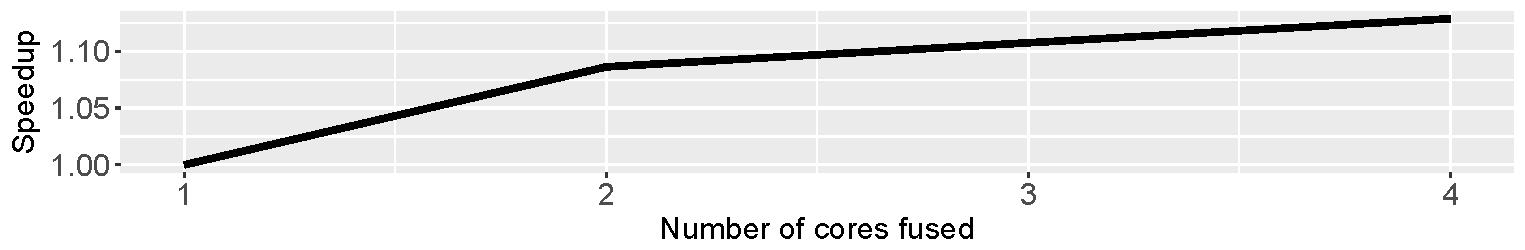
\includegraphics[width=1\textwidth]{chapter3/graphics/mser_branch_motiv.pdf}

    \caption{Performance of \bm{MSER} using the currently implemented branch predictor vs a perfect branch predictor.}
    \label{fig:mser_motiv}
	\vspace{1em}
\end{figure}

In this section, perfect branch prediction is explored on the \bm{MSER} benchmark as it is a perfect candidate for evaluating branch prediction accuracy improvements.
Figure~\ref{fig:mser_motiv} shows the execution time (in cycles) of \bm{MSER} on two different core composition sizes, 2 and 4.
The speedup is obtained by comparing the performance to a single core with perfect branch prediction.
As the figure shows, modifying the accuracy leads to a performance increase of 10\% on a 4 core composition.
Whilst this increase may appear small, it already demonstrates that branch prediction can help improve performance.

The reason performance does not improve drastically is still due to the fact that \bm{MSER} features small blocks.
As seen in Chapters~\ref{chp:streamit} and ~\ref{chp:cases}, programs that feature small blocks do not perform well on core compositions due to the fact that they increase the branch prediction accuracy requirements and increase synchronisation costs.
However, this is also due to the fact that core compositions fetch blocks in a sequential fashion, which may impede performance.

\subsection{Fetching mechanism}

%Chapter~\ref{chp:cases} demonstrated how block size affects the performance of core composition, due to the fact that it increases the cost of synchronization and puts a strain on branch prediction.
%Whilst the chapter focused on the size of blocks, it is not the sole determining factor of whether or not a set of blocks may be executed efficiently on a core composition.
%For example, a small block containing load operations can potentially take at least 100 cycles to execute due to a cache miss.
%In such a situation, the execution of the small block covers the latency caused by fetching multiple blocks on a large composition.
%Thus, small blocks that take a long time to execute can benefit from core composition as long as the branch prediction is accurate.
%Therefore, another feature to take into account when considering core composition is average execution time of a block.

In the current core composition scheme (see Chapter~\ref{chp:Background} for more details), cores fetch in a serial fashion.
When a core composition is initiated, one of the cores will start fetching blocks until its instruction window is full.
Once the instruction window is full, the core will submit a fetch request to another core in the composition, which will then repreat the procedure.
However, if a block in the currently fetching core were to commit before the instruction window is full, the core will never submit a fetch request to another core.
In this situation, cores in a composition may remain inactive during the execution of a program.

\begin{figure}[t]
    \centering
    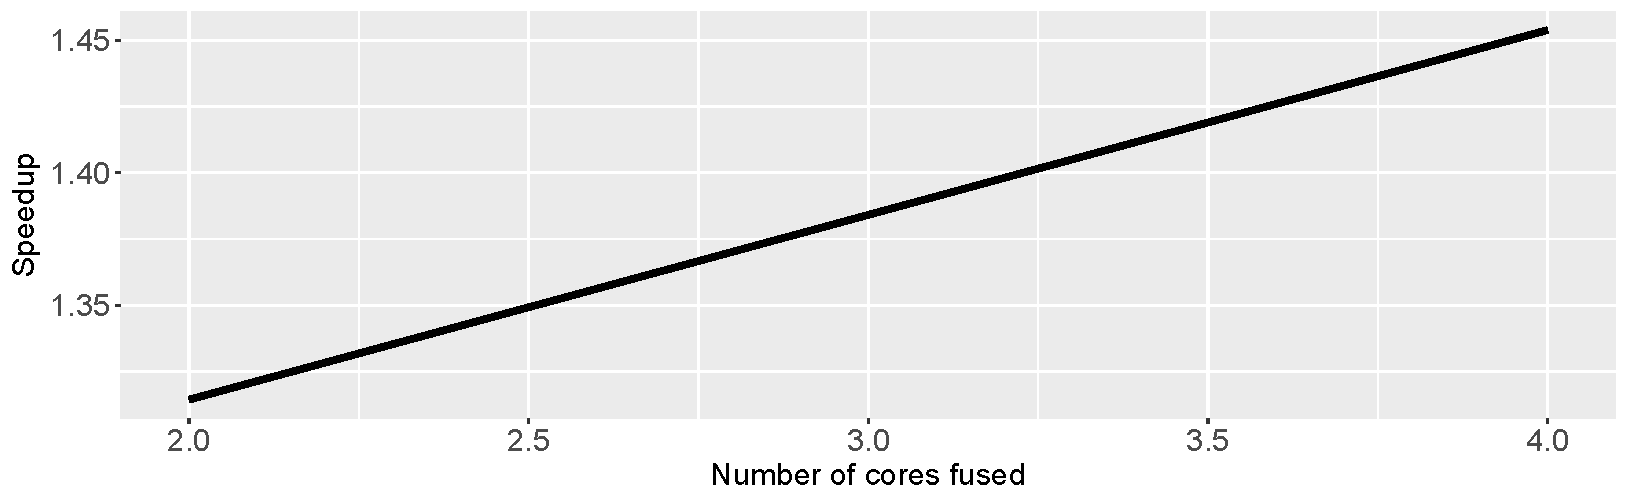
\includegraphics[width=1\textwidth]{chapter3/graphics/motiv_mser_fetch.pdf}
    \caption{Speedup obtained when executing the MSER benchmark on 2 and 4 core composition with the new fetching scheme. Higher is better.}
    \label{fig:motivation_fetch}
	\vspace{1em}
\end{figure}

Figure~\ref{fig:motivation_fetch} illustrates how a new fetching mechanism can improve the performance of the \bm{MSER} benchmark using perfect branch prediction.
The baseline is a single core with perfect branch prediction.
The figure shows that with the new scheme, a 4 core composition can improve performance by 1.45x, compared to the 1.15x of using the old fetching scheme.
In essence, the new fetching scheme aims to reduce the amount of communication between cores by allowing cores to fetch independently.

To further motivate the use of a new fetching scheme, it is important to consider how often all the cores in a composition are being used.
As previously stated, in the current model, serialisation may cause certain cores to be empty for a long amount of time, due to the fact that other cores in the composition are never filling their instruction windows.
To understand how this can affect the average amount of time a core is executing code, the simulator tracks the number of cycles a core has live instructions in its window, these are called \textit{active cycles}.

\begin{figure}[t]
    \centering
    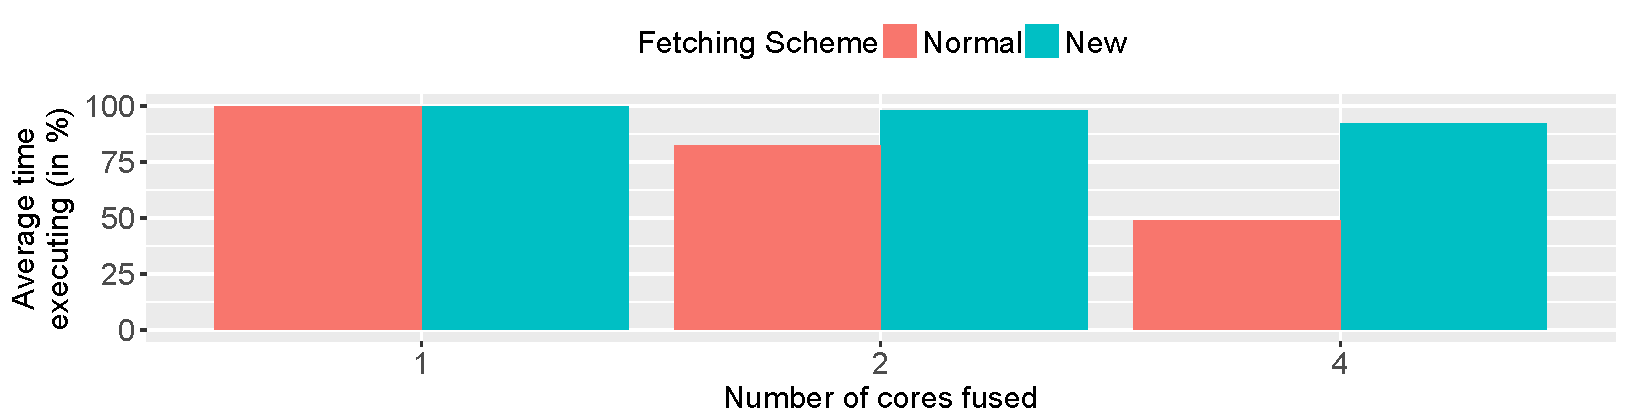
\includegraphics[width=1\textwidth]{chapter3/graphics/fetch_av_time.pdf}
    \caption{Percentage of time (in cycles) cores in a composition are executing instructions compared to the overall execution time. Higher is better.}
    \label{fig:motivation_perc}
	\vspace{1em}
\end{figure}

Figure~\ref{fig:motivation_perc} compares the average \textit{active cycles} of a core in a 2 and 4 core composition on the \bm{MSER} benchmark with and without the new fetching scheme.
The average is obtained by taking the \textit{active cycles} of each core in the composition, averaging them, and then comparing it to the overall execution time of the benchmark.
The figure shows that with the normal fetching scheme on a 4 core composition, cores are active only 50\% of the total execution time, compared to 92\% on the new fetching scheme.

Overall, Figure~\ref{fig:motivation_perc} demonstrates that the current fetching model is inadequate when blocks are small and execute quickly.
Whilst this was illustrated in previous chapters, this Section has demonstrated that modifying the fetching scheme can in fact improve the overall performance of core composition on blocks that were previously considered incompatible with core composition.
The uneven active execution time seen in the normal fetching scheme are caused by the serialisation of fetches, which increases the reliance on inter-core communication.
Thus it is important to find new methods of fetching blocks that reduce communication.

\subsection{Register dependencies}

In EDGE, global registers are only used for inter-block communication.
When multiple blocks are in flight, if a block requires to read a register that will be written to by an older block, it must naturally wait until that write has been execute.
Thus when executing multiple blocks in parallel data dependencies may arise.
This can be especially problematic when core composition is used, as up to 64 blocks could potentially be in flight at any moment.
If the data dependencies are not resolved quickly enough, then this causes blocks to execute in a serial fashion, which may reduce any potential benefit from using the composition.

The register dependency issue is a common problem for superscalar processors~\cite{} where ILP is limited by data-dependencies.
One solution to the problem of data-dependencies is adding a value predictor to the processor.
To summarize Section~\ref{} of Chapter~\ref{chp:Background}, value predictors predict data at specific addresses, in a similar fashion to branch predictors.
This allows instructions to execute with speculative data, and thus decrease the penalty caused by data-dependencies.
In cases where data is modified in a regular way, value predictors 
Whilst the register dependencies found in Listing~\ref{lst:bloop} are problematic, they can be resolved through the use of a value predictor.

\begin{figure}[t]
    \centering
    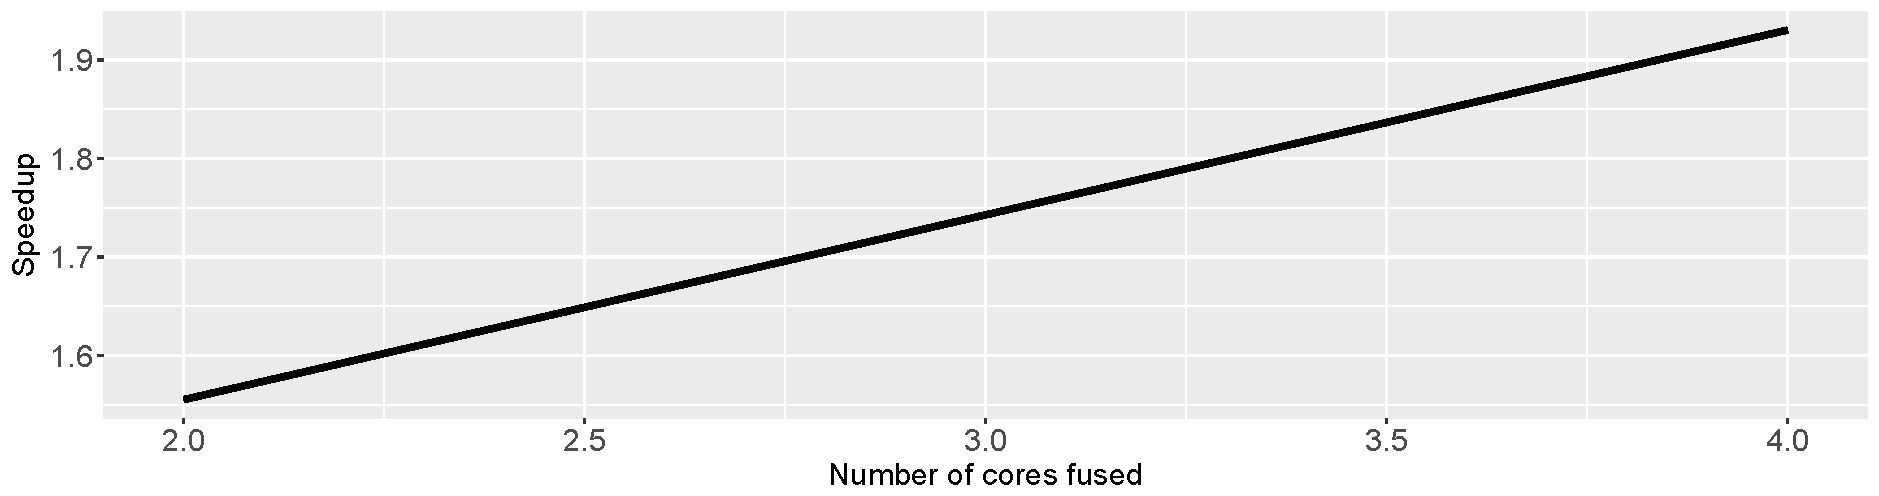
\includegraphics[width=1\textwidth]{chapter3/graphics/mser_fetch_motiv.pdf}

    \caption{Speedup of executing \bm{MSER} using the new fetching mechanism, with perfect value prediction and perfect branch prediction. Higher is better.}
    \label{fig:motivation_reg}
	\vspace{1em}
\end{figure}

Figure~\ref{fig:motivation_reg} shows the performance of executing \bm{MSER} with perfect value prediction on core compositions of size 2 and 4 using the new fetching scheme with perfect branch prediction.
The speedup is obtained by comparing the execution time of core compositions to a single core with perfect branch prediction and perfect value prediction.
As shown in the Figure, a 4 core composition can now get a speedup of 1.93x, compared to the 1.45x when using only perfect branch prediction and the new fetching scheme.
This is due to the fact that register dependencies are no longer serialising the computation between blocks, and thus blocks can be executed almost entirely in parallel.


\subsection{Putting it all together}

The previous 3 sections demonstrate that with modifications of the hardware, a previous benchmarks that showed very little performance gains with core composition can now see a performance increase of up to 1.90x on a 4 core composition.
This demonstrates that the hardware used for core composition can be improved in order to tackle difficult applications.
Whilst the previous three sections accumulated hardware modifications to obtain the 1.90x speedup, it is important to show how all these changes must be included in the processor in order to obtain the best results.

\begin{figure}[t]
    \centering
    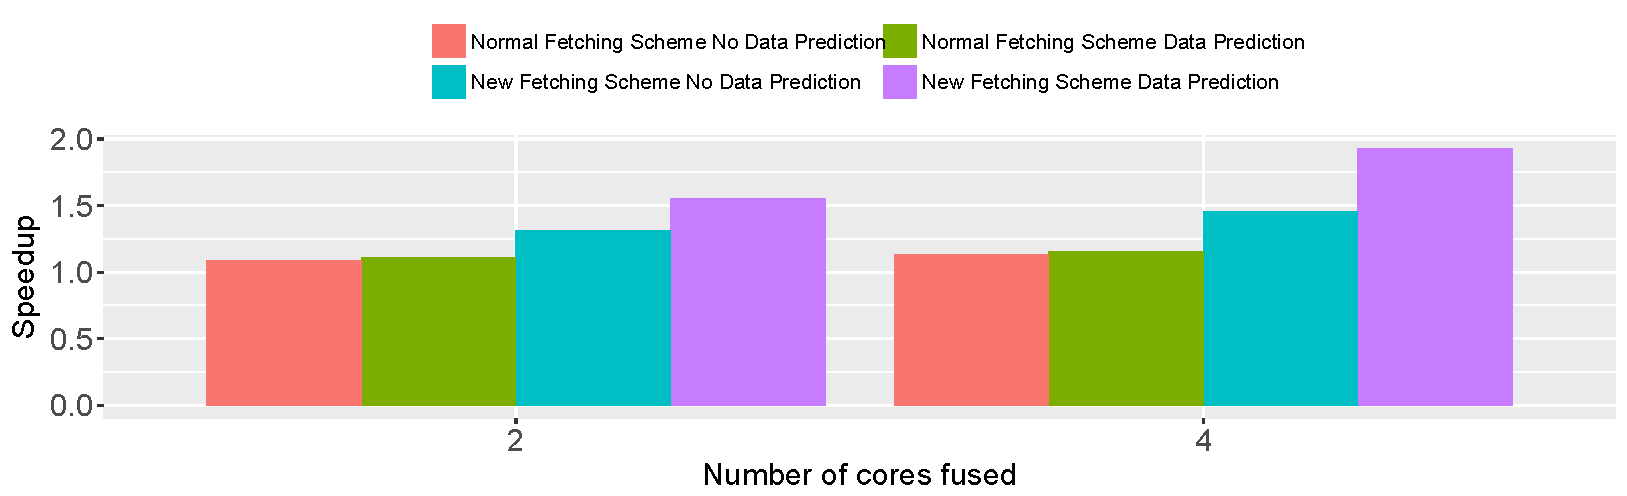
\includegraphics[width=1\textwidth]{chapter3/graphics/mser_final_motiv.pdf}
    \caption{Speedup obtained when executing the MSER benchmark on 2 and 4 core composition with the new fetching scheme. Higher is better.}
    \label{fig:motivation_final}
	\vspace{1em}
\end{figure}

Figure~\ref{fig:motivation_final} shows how the performance of \bm{MSER} is improved on when adding either the new fetching scheme, the value predictor, or both.
The performance is compared to a single core with or without value prediction.
Overall, the figure reveals that the current fetching scheme -- even with perfect value prediction and perfect branch prediction -- cannot obtain any significant performance improvements.
This is due to the fact that the core compositions are limited by the serialisation of block fetches.
Adding value prediction does not improve performance greatly because of the fact that it reduces the execution time of blocks, which once again increases the difficulty of populating cores with blocks.

On the other hand, the figure also highlights that modifying the fetching scheme does not suffice in order to get the fastest execution times.
This is due to the fact that if cores are able to fetch blocks at a much faster rate, they will then be limited by potential register dependencies.
Therefore, it is important to consider multiple modifications to the hardware in order to get the best performance.

Finally, it is important to remember that these results are currently only made possible through the use of perfect branch prediction.
Executing \bm{MSER} without perfect branch prediction leads to an average accuracy of 86\%, which is not enough to ensure that core composition can be efficiently used.
This motivates exploring the potential performance of core composition through the use of a perfect branch predictor.
